\documentclass[a4paper, 12pt, oneside, openright]{article}

%##### Packages, Settings

\usepackage[main=ngerman, english]{babel}

\usepackage{lipsum}
\usepackage{acronym}
\usepackage{graphicx}
\graphicspath{ {./Bilder/} }
\usepackage{caption}
\usepackage[backend=bibtex,style=alphabetic,citestyle=authoryear]{biblatex} %Imports biblatex package
\addbibresource{Literaturverzeichnis.bib} %Imports bibliography file
\usepackage{inputenc}
% letztes package
\usepackage[hidelinks]{hyperref}
\addto\extrasngerman{\def\figureautorefname{Abbildung}}
\usepackage{placeins}

%##### Start

\begin{document}

%##### Title Seite
\begin{titlepage}
\begin{center}
\centering

\includegraphics[scale=0.3]{thi_logo_wb_RGB}\\
\vspace{1.5cm}
\textbf{\large Bachelorarbeit\\}
\vspace{0.5cm}
\textbf{\LARGE Titel}\\
\vspace{1.0cm}
\textbf{zur Erlangung des akademischen Grades eines\\Bachelor of Science\\}
\vspace{2.0cm}
\textbf{angefertigt von\\Vorname Name\\}
\vspace{2.0cm}
\textbf{Betreuer:\\}
\vspace{0.5cm}
\begin{tabular}{l l}
Erstprüfer & Betreuer A\\
Zweitprüfer & Betreuer B\\           
\end{tabular}\\
\vspace{0.5cm}
ausgegeben am \\
abgegeben am \\
\vfill
Hochschulname\\
Fakultät\\
Studiengang\\
\end{center}
\end{titlepage}

%##### Erklärung
\pagenumbering{Roman}
\phantomsection
\addcontentsline{toc}{section}{Erklärung}
\textbf{\Large Erklärung}
\vspace{1.0cm}\\
% NAME !!!!!!!!!!!!!!!!!!!!!!!!!!!!!
Hiermit erkläre ich, NAME, dass ich die vorliegende Bachelorarbeit bis auf die offizielle
Betreuung selbstständig und ohne die Hilfe von Dritten verfasst habe. Die Arbeit wurde noch
nicht für anderweitige Prüfungszwecke vorgelegt.
Die verwendeten Quellen sowie die verwendeten Hilfsmittel sind vollständig angegeben. Wörtlich
übernommene Textteile und übernommene Bilder und Zeichnungen sind in jedem Einzelfall
kenntlich gemacht.
\vspace{2.0cm}\\


\begin{tabular}{@{}p{6cm}p{6cm}@{}}
Ort, Datum & \hrulefill \\
& Name \\
\end{tabular}

                              
\newpage

%##### Danksagung
\phantomsection
\addcontentsline{toc}{section}{Danksagung} 
\textbf{\Large Danksagung}\\
\vspace{0.5cm}\\
\textbf{Person A} \\\\
\textbf{Person B} \\\\
\newpage

%##### Abkürzungsverzeichnis
\phantomsection
\addcontentsline{toc}{section}{Abkürzungsverzeichnis} 
\textbf{\Large Abkürzungsverzeichnis}\\
\begingroup
\setlength{\labelsep}{1cm}
\begin{acronym}[XXXXXX]
%\acro{Kürzel}[Kurzform]{Langform}
\acro{API}[API]{Application Programming Interface}
% Verwendung von Abkürzungen
% \ac{API}
\end{acronym}
\endgroup
\newpage

%##### Abbildungsverzeichnis
\phantomsection
\addcontentsline{toc}{section}{Abbildungsverzeichnis} 
\listoffigures
\newpage

%##### Inhaltsverzeichnis
\phantomsection
\addcontentsline{toc}{section}{Inhaltsverzeichnis}
\tableofcontents
\newpage

%##### Abstrakt
\setcounter{page}{1}
\pagenumbering{arabic}
\section{Abstrakt}
Hier steht das Abstrakt.
\newpage

%##### Kapitel 2
\section{Kapitel 2}

\begin{figure}[!h]
\centering
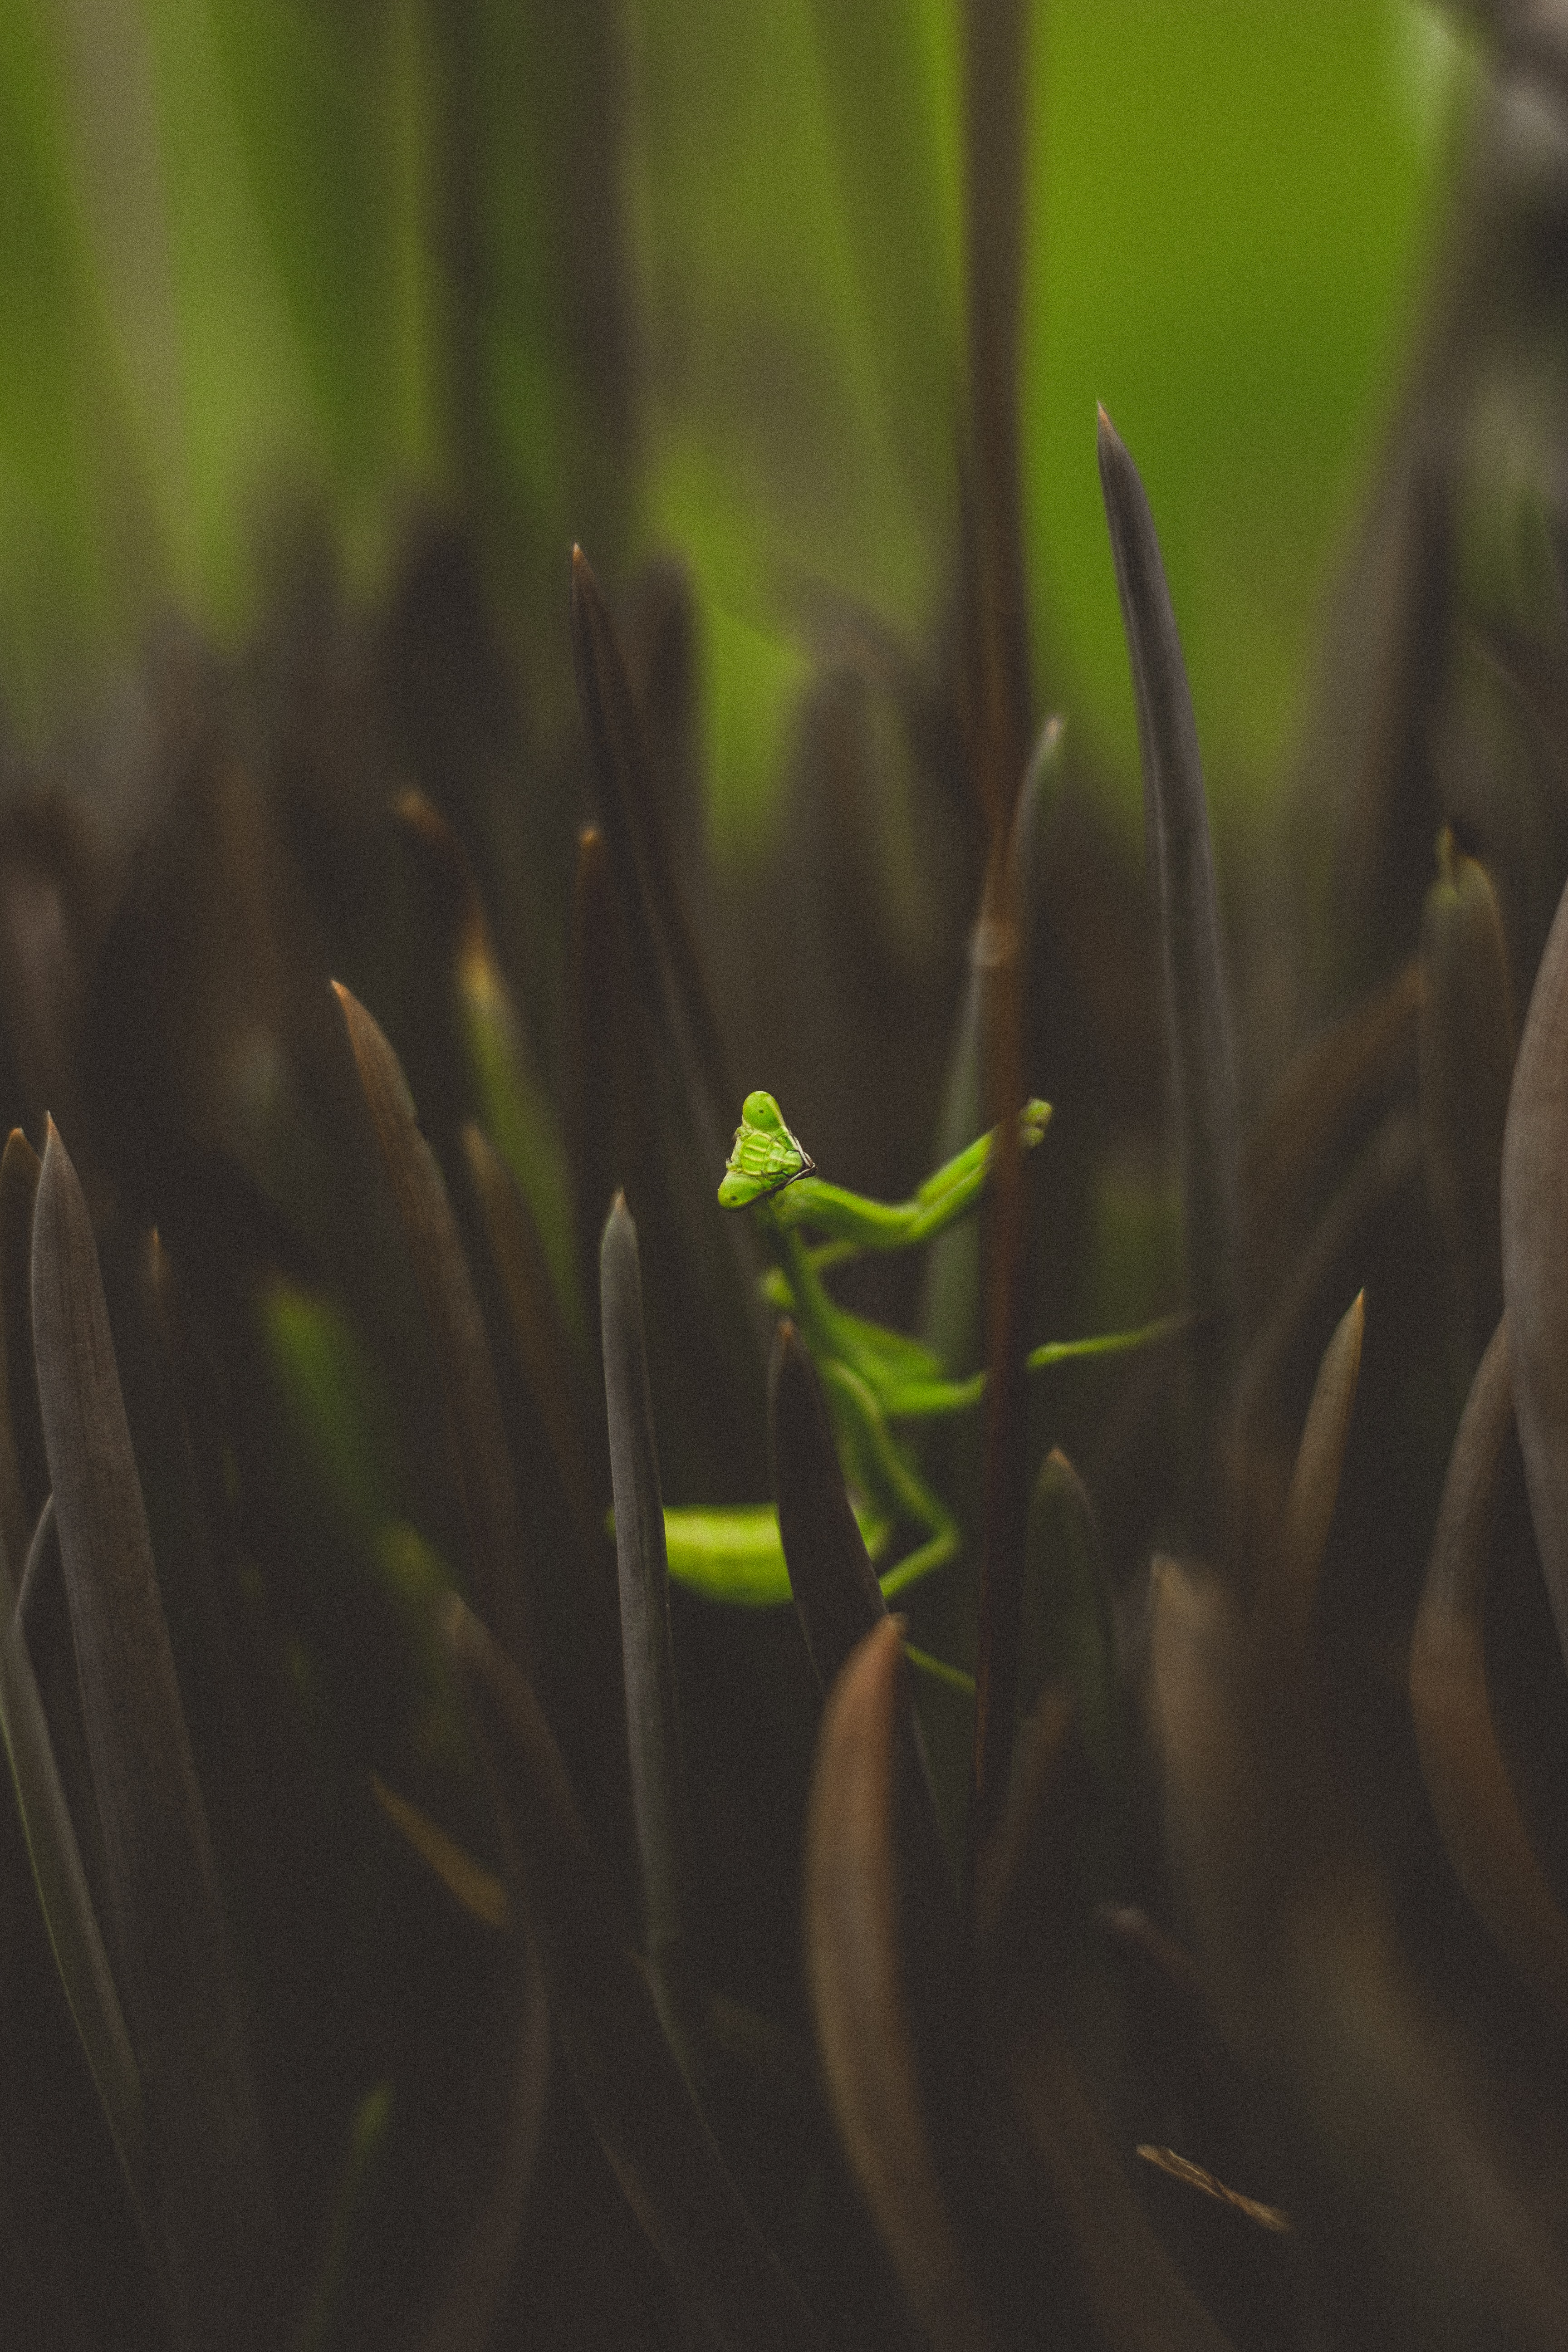
\includegraphics[scale=0.05]{geronimo-giqueaux-dalwoqwFUZQ-unsplash}
\caption{Ein tolles Bild}
\label{geronimo-giqueaux-dalwoqwFUZQ-unsplash}
\end{figure}

Auf \autoref{geronimo-giqueaux-dalwoqwFUZQ-unsplash} sieht man ein Tier.\\
Das Bild ist von \href{https://unsplash.com/@ggiqueaux}{unsplash.com/@ggiqueaux}.\\
Das ist ein Zitat (\cite[vgl.][S. 10]{misc}).\\
Was ist eine \ac{API}?\\

%##### Unterkapitel 2.1
\subsection{Unterkapitel 2.1}
% dummy text
\lipsum[1]

%##### Unterkapitel 2.2
\subsection{Unterkapitel 2.2}

%##### Kapitel 3
\section{Kapitel 3}

%##### Unterkapitel 3.1
\subsection{Unterkapitel 3.1}

%##### Unterkapitel 3.2
\subsection{Unterkapitel 3.2}

\section{Fazit und Ausblick}
Hier steht das Fazit.

\newpage

%##### Literaturverzeichnis
\pagenumbering{Roman}
% Der Counter muss manuell gesetzt werden !!!!!!!!!!!!!!!!!!!!!!!!
\setcounter{page}{6}
\phantomsection
\addcontentsline{toc}{section}{Literaturverzeichnis}
\printbibliography[title={Literaturverzeichnis}]

\end{document}